\section{Différents conditionnements pour des médicaments (11 points)}

Trois médicaments sont proposés sous différents conditionnements :


Le premier médicament $M_1$ est proposé en ampoules $(A)$, en comprimés $(C)$ ou en gélules $(G)$.

Le deuxième médicament $M_2$ est proposé en ampoules $(A)$ ou en comprimés $(C)$.

Le troisième médicament $M_3$ est proposé en comprimés $(C)$ ou en gélules $(G)$.\\

Une personne achète d'abord $M_1$ puis $M_2$ puis $M_3$ en laissant le hasard décider du conditionnement.\\


On note dans l'ordre les choix respectifs pour $M_1$, $M_2$ et $M_3$.
Par exemple le choix $CAG$ signifie que :
\begin{itemize}
	\item $M_1$ est sous forme de Comprimés;
	\item $M_2$ est sous forme d'Ampoules;	
	\item $M_3$ est sous forme de Gélules.
\end{itemize}

\subsection{}
\begin{questions}
	\question[2] Donner les 12 choix possibles. On pourra s'aider d'un arbre.
	\begin{solution}
		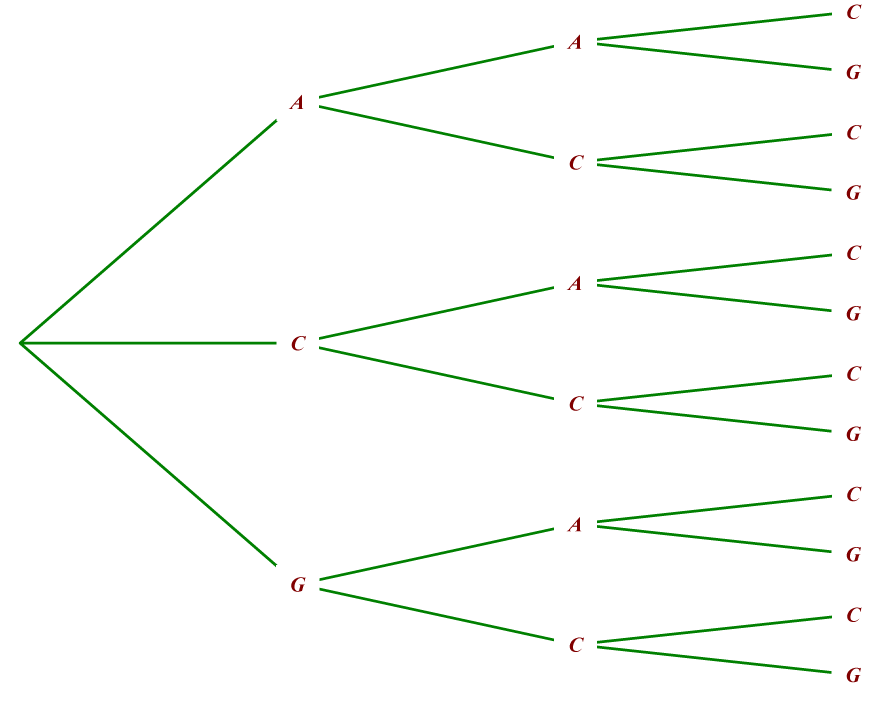
\includegraphics[scale=0.5]{arbre}
		
		Les 12 choix possibles sont : $AAC$, $AAG$, $ACC$, $ACG$, $CAC$; $CAG$, $CCC$; $CCG$ , $GAC$, $GAG$, $GCC$; $GCG$.
	\end{solution}
	
	\question[5] Donner les choix correspondants aux événements suivants :
	
	\begin{itemize}
		\item[$E_1$ :]  << Les trois médicaments sont délivrés sous forme de comprimés>>;
		\item[$E_2$ :] << Deux médicaments exactement sont délivrés sous forme de comprimés>>;
		\item[$E_3$ :] << Les trois médicaments sont délivrés sous trois conditionnements différents>>;
		\item[$E_4$ :] << $M_1$ est délivré sous forme de comprimés et $M_2$ sous forme de gélules>>;
		\item[$E_5$ :] << $M_1$ est délivré sous forme de comprimés ou $M_3$ sous forme de gélules>>;
	\end{itemize}

	\begin{solution}
		\begin{itemize}
			\item Le choix correspondant à l'événement $E_1$ est : $CCC$.
			\item Les choix correspondants à l'événement $E_2$ sont : $ACC$, $CAC$, $CCG$ et $GCC$.
			\item Les choix correspondants à l'événement $E_3$ sont : $ACG$, $CAG$ et $GAC$.
			\item Aucun choix ne correspond à l'événement $E_4$.
			\item Les choix correspondants à l'événement $E_5$ sont : $CAC$, $CAG$, $CCC$, $CCG$, $AAG$, $ACG$, $GAG$, $GCG$.
		\end{itemize}
	\end{solution}
\end{questions}

\subsection{}

On suppose que tous les choix sont équiprobables. On donnera les résultats sous forme de fractions irréductibles.

\begin{questions}
	\question[1] Calculer la probabilité $P(E_1)$ de l'événement $E_1$.
	\begin{solution}
		$P(E_1)=\dfrac{1}{12}$
	\end{solution}
	
	\question[1] Montrer que $P(E_2)=\dfrac{1}{3}$.
	 \begin{solution}
	 	$P(E_2)=\dfrac{4}{12}=\dfrac{1}{3}$.
	 \end{solution}
	
	\question[2] Calculer de même $P(E_3)$ ; $P(E_4)$ ; $P(E_5)$.
	\begin{solution}
		\begin{eqnarray*}
			P(E_3) &=& \dfrac{3}{12} = \dfrac{1}{4} \\
			 & & \\
			P(E_4) &=& \dfrac{0}{12} = 0 \\
			& & \\
			P(E_5) &=& \dfrac{8}{12} = \dfrac{2}{3} 
		\end{eqnarray*}
	\end{solution}
\end{questions} 